%----------------------------------------------------------------------------
\section{Formal Verification}\label{sec:formal_verification}
%----------------------------------------------------------------------------

In order to raise the reliability of system analysis, a system analysis technique is required that can have the precision of paper-and-pencil based mathematical proofs, and thus does not rely upon computer-arithmetic, and utilizes the computers for bookkeeping, to be able to handle complex systems without having to worry about human-errors. Formal verification methods, which are primarily based on theoretical computer science fundamentals like logic calculi, automata theory and strongly type systems, fulfil these requirements. The main principle behind formal analysis of a system is to construct a computer based mathematical model of the given system and formally verify, within a computer, that this model meets rigorous specifications of intended behaviour. Due to the mathematical nature of the analysis, 100\% accuracy can be guaranteed.\cite{https://doi:10.4018/978-1-4666-5888-2.ch705}

\subsection{Model Checking}

\emph{Model Checking} is a formal verification method to verify properties of finite systems, i.e., to decide whether a given formal model \(M\) satisfies a given requirement \(\gamma\) or not. The name comes from formal logic, where a logical formula may have zero or more models, which define the interpretation of the symbols used in the formula and the base set such that the formula is true. In this sense, the question is whether the formal model is indeed a model of the formal requirement: \(M \models \gamma\)?

Model Checker algorithms (see \autoref{fig:model_checking}), such as UPPAAL\footnote{https://uppaal.org/}\cite{uppaal} or Theta\footnote{https://inf.mit.bme.hu/en/theta}\cite{theta} use SAT solvers to answer this question; and can even return a \emph{proof} (i.e., a part of the model) that \(M\) indeed does satisfy said requirement\footnote{These proofs usually come in the form of an execution trace}.

\begin{figure}[!ht]
	\centering
	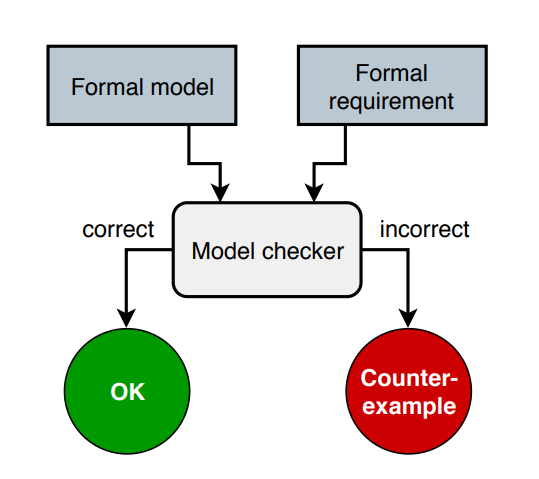
\includegraphics[width=67mm, keepaspectratio]{figures/model_checking.png}\hspace{1cm}
	\caption{An illustration of model checking.}
	\label{fig:model_checking}
\end{figure}

\subsection{Petri Net}\label{ssec:petri-net}

\begin{figure}[!ht]
	\centering
	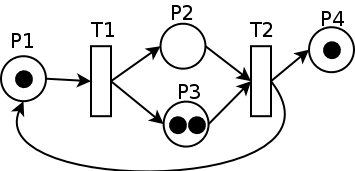
\includegraphics[width=67mm, keepaspectratio]{figures/petri_net.png}\hspace{1cm}
	\caption{An example Petri net with 2 transitions and 4 places.}
	\label{fig:petri_net}
\end{figure}

Petri nets are a widely used formalism to model concurrent, asynchronous systems \cite{24143}. The formal definition of a Petri net (including inhibitor arcs) is as follows (see \autoref{fig:petri_net} for an illustration of the notations).

\begin{definition}[Petri net]
	
	A Petri net is a tuple \( PN = (P, T, W, M_0) \)
	
	\begin{itemize}
		\item \(P\) is the set of \emph{places} (defining state variables);
		\item \(T\) is the set of \emph{transitions} (defining behaviour), such that \( P \bigcap T = \emptyset \);
		\item \(W \subseteq W^+ \bigcup W^- \) is a set of two types of arcs, where \(  W^+ : T \times P \rightarrow \mathbb{N}\) and \( W^- : P \times T \rightarrow \mathbb{N} \) are the set of input arcs and output arcs, respectively (\( \mathbb{N} \) is the set of all natural numbers);
		\item \(M_0 : P \rightarrow \mathbb{N} \) is the \emph{initial marking}, i.e., the number of \emph{tokens} on each place.
	\end{itemize}
\end{definition}

The state of a Petri net is defined by the current marking \( M : P \rightarrow \mathbb{N} \). The behaviour of the systems is described as follows. A transition \( t \) is enabled if \( \forall p \in P : M(p) \in W(p, t) \). Any enabled transition \(t\) may fire non-deterministically, creating the new marking \( M' \) of the Petri as follows: \( \forall p \in P : M'(p) = M(p) - W^-(p, t) + W^+(t, p) \).

In words: W describes the \emph{weight} of each flow from a transition to a place, or from a place to a transition. Firing a transition \(t\) in a marking \(M\) consumes \(W^-(p_i, t)\) tokens from each of its input places \(p_i\), and produces \(W(t, p_o)\) tokens in each of its output places \(p_o\). One such transition \(t\) is \emph{enabled} (it may \emph{fire}) in \(M\) if there are enough tokens in its input places for the consumptions to be possible, i.e., if and only if \( \forall p : M(p) \ge W(s, t)\).

\subsection{Activities as Petri Nets}\label{ssec:activities-as-petri-nets}

Formal verification requires models to be specified using \emph{mathematical} precision. The paper called "Verifying SysML activity diagrams using formal transformation to Petri nets"\cite{https://doi.org/10.1002/sys.21524} by Edward Huang, Leon F. McGinnis and Steven W. Mitchell proposes a way to \emph{partially} map SysML activity diagrams to Petri nets. In the following, I will summarise their work.

\subsubsection{Constrained Sub-set of SysML}\label{ssec:sysml_assumptions}

Since SysML Activity Diagrams do not have exact execution semantics\cite{euml}, the PN mapping can only be done for a limited subset of the modeling elements: \emph{actions}, \emph{initial nodes}, \emph{final nodes}, \emph{join nodes}, \emph{fork nodes}, \emph{merge nodes}, \emph{decision nodes}, \emph{pins} and \emph{object/control flows}, which have precise execution semantics as defined in the Foundational Subset for Executable UML Models.\cite{fuml}

The paper also assumes the following constrains:

\begin{enumerate}
	\item The value of tokens is not considered.
	\item Control flows with multiple tokens at a time are not considered.
	\item Optional object/control flows are not considered, ie, multiplicity lower bounds are strictly positive.
\end{enumerate}

These constraints allow the mapping between activities and Petri nets, however, the constructed PN will not be semantically equivalent - data cannot flow between nodes. This fact will be addressed in \autoref{ch:activiy_verification}.

\subsubsection{Mapping Rules}

Activity elements can be grouped into two sets: \emph{load-and-send} (LAS) and \emph{immediate-repeat} (IR).

LAS nodes are fired when all their inputs have tokens. When an LAS node fires, the number of tokens associated with the input arcs/pin is consumed and the number of tokens associated with an output arc/pin is added. In SysML activity diagrams, the execution semantics of fork nodes, join nodes, and basic actions are also LAS because these nodes are fired when all their input nodes have at least one token. As a result, these nodes can be mapped to \emph{transitions} in the resulting Petri net.

In contrast, as soon as an IR node receives a token from any input, it immediately adds a token to its output nodes. For UML/SysML activity diagrams, activity final nodes, merge nodes, decision nodes and pins are IR nodes because they are fired immediately when any token is received. As a result, these nodes can be mapped to \emph{places} in the resulting Petri net.

Given the set of assumptions in \autoref{ssec:sysml_assumptions}, control flows and object flows in an activity diagram can be mapped to arcs in a Petri net.

Thus, we have defined how to map the constrained set of Activity Diagram elements to Petri net elements.

\subsubsection{Example Mapping}

Figure ... shows an example mapping from a SysML activity diagram to a Petri net

For more information, please refer to the Paper!